\subsection{Team congregation}	
\subsubsection{29.09.14}

\begin{enumerate}
	\item The time of beginning and ending of the congregation: 18:00 - 21:30
	\item Purposes of the congregation:
	\begin{enumerate}
	  \item Discuss the rules of FTC Cascade Effect.
	  
	  \item Discuss the main aspests of robot's construction.
	  
      \item Elaborate strategy of our team's play. 
    \end{enumerate}
	\item Work, that has been done
	\begin{enumerate}
	  \item  Was discussed in part 2 of rules.
	  
	  \item During the discussion of construction of robot there have been several ideas: 
	  \begin{enumerate}
	    \item Dimensions of the robot:
	    \begin{enumerate}
	      \item Robot must be compact enough in addition to body of robot in size to fit gripper of  balls.
	      
	      \item Robot must be compact to don't prevent to alliance partner.
	      
	      \item Body of robot mustn't be too small,otherwise t will be unstable when the lift is raised to maximum height (120cm)
	      
	    \end{enumerate}
	    
	    \item Wheel base:
	    \begin{enumerate}
	      \item Construction with four standard wheels from set Tetrix. This system can move in a straight and turn on the spot very good. A minor defect of this construction is that when turning of robot wheels jump and robot shakes.  
	      
	      \item Construction with two caterpillars. This construction has advantage that it can move in a straight and turn on the spot. The disadvantage of this system that caterpillar can get off. In addition caterpillars there is no in Tetrix set so we must make to their ourself.  
	      
	      \item Construction with four omni wheels from Tetrix set that located at angle of 45 degrees to the body of robot. The advantage of this construction that it can move to any direction and can turn very fast but move in a straight badly that could adversely affect the Autonomous period.
	      
	      \item Construction with four mechanum wheels that located as standard wheels. Advantages: good moving in a straight, fast turning, opportunity of moving to any direction. Disadvantages: the need buy this wheels, low accuracy on turning.
	      
	      \begin{figure}[h]
	      	\begin{minipage}[h]{0.165\linewidth}
	      		\center  
	      	\end{minipage}
	      	\begin{minipage}[h]{0.6\linewidth}
	          \center{\includegraphics[scale=0.3]{days/29.09.14/images/01}}
	          \caption{Ideas of wheel base: 1)Construction with four standard wheels 2)Construction with two caterpillars 3) Construction with four omny wheels from Tetrix set 4)Construction with four mechanum wheels}
	        \end{minipage}
	      \end{figure}
	      
	    \end{enumerate}
	    
	    \item System of control of balls:
	    \begin{enumerate}
	      \item Basket for balls fixed to system of retractable slats that interconnected  with help servomotors. Advantages: the absence of a line that can tear. Disadvantages: the complexity and low reliability.	
	      
	      \item Basket for balls fixed to system of retractable slats that fixed to body of robot. Extracting lift by using DC-motors that reel up the line. Advantages: simple and reliability (except for the line). Disadvantages: line can tear.
	      
	      \item Basket for balls fixed to system of retractable slats that fixed to DC motor that capable of rotating slats in the vertical plane. Advantages: opportunity of extracting in horizontal position that relieves the load from the line. Disadvantages: line can tear.
	      \begin{figure}[H]
	      	\begin{minipage}[h]{0.2\linewidth}
	      		\center  
	      	\end{minipage}
	      	\begin{minipage}[h]{0.6\linewidth}
	      		\center{\includegraphics[scale=0.3]{days/29.09.14/images/02}}
	      		\caption{Ideas of the lift 1)Construction №1 2)Construction with stationary slats 3) Construction with slats that fixed to DC motor}
	      	\end{minipage}
	      \end{figure}
	      
	    \end{enumerate}
	    
	    \item System of fixing of moving basket (for more accurate moving of balls to basket and for moving of it):
	    \begin{enumerate}
	      \item Gripper shaped П with two servomotors that fixes basket between the beams, located at DC motor that can rotate it in vertical plane. Advantages: opportunity of raise basket. Disadvantages: takes a lot of space.
	      
          \item The same gripper but instead beams-claws use the hooks that can capture basket for small holes in its base. Advantages: more compact than previous variant. Disadvantages: to get the hooks into the holes will be difficult.
			\begin{figure}[H]
				\begin{minipage}[h]{0.2\linewidth}
					\center  
				\end{minipage}
				\begin{minipage}[h]{0.6\linewidth}
					\center{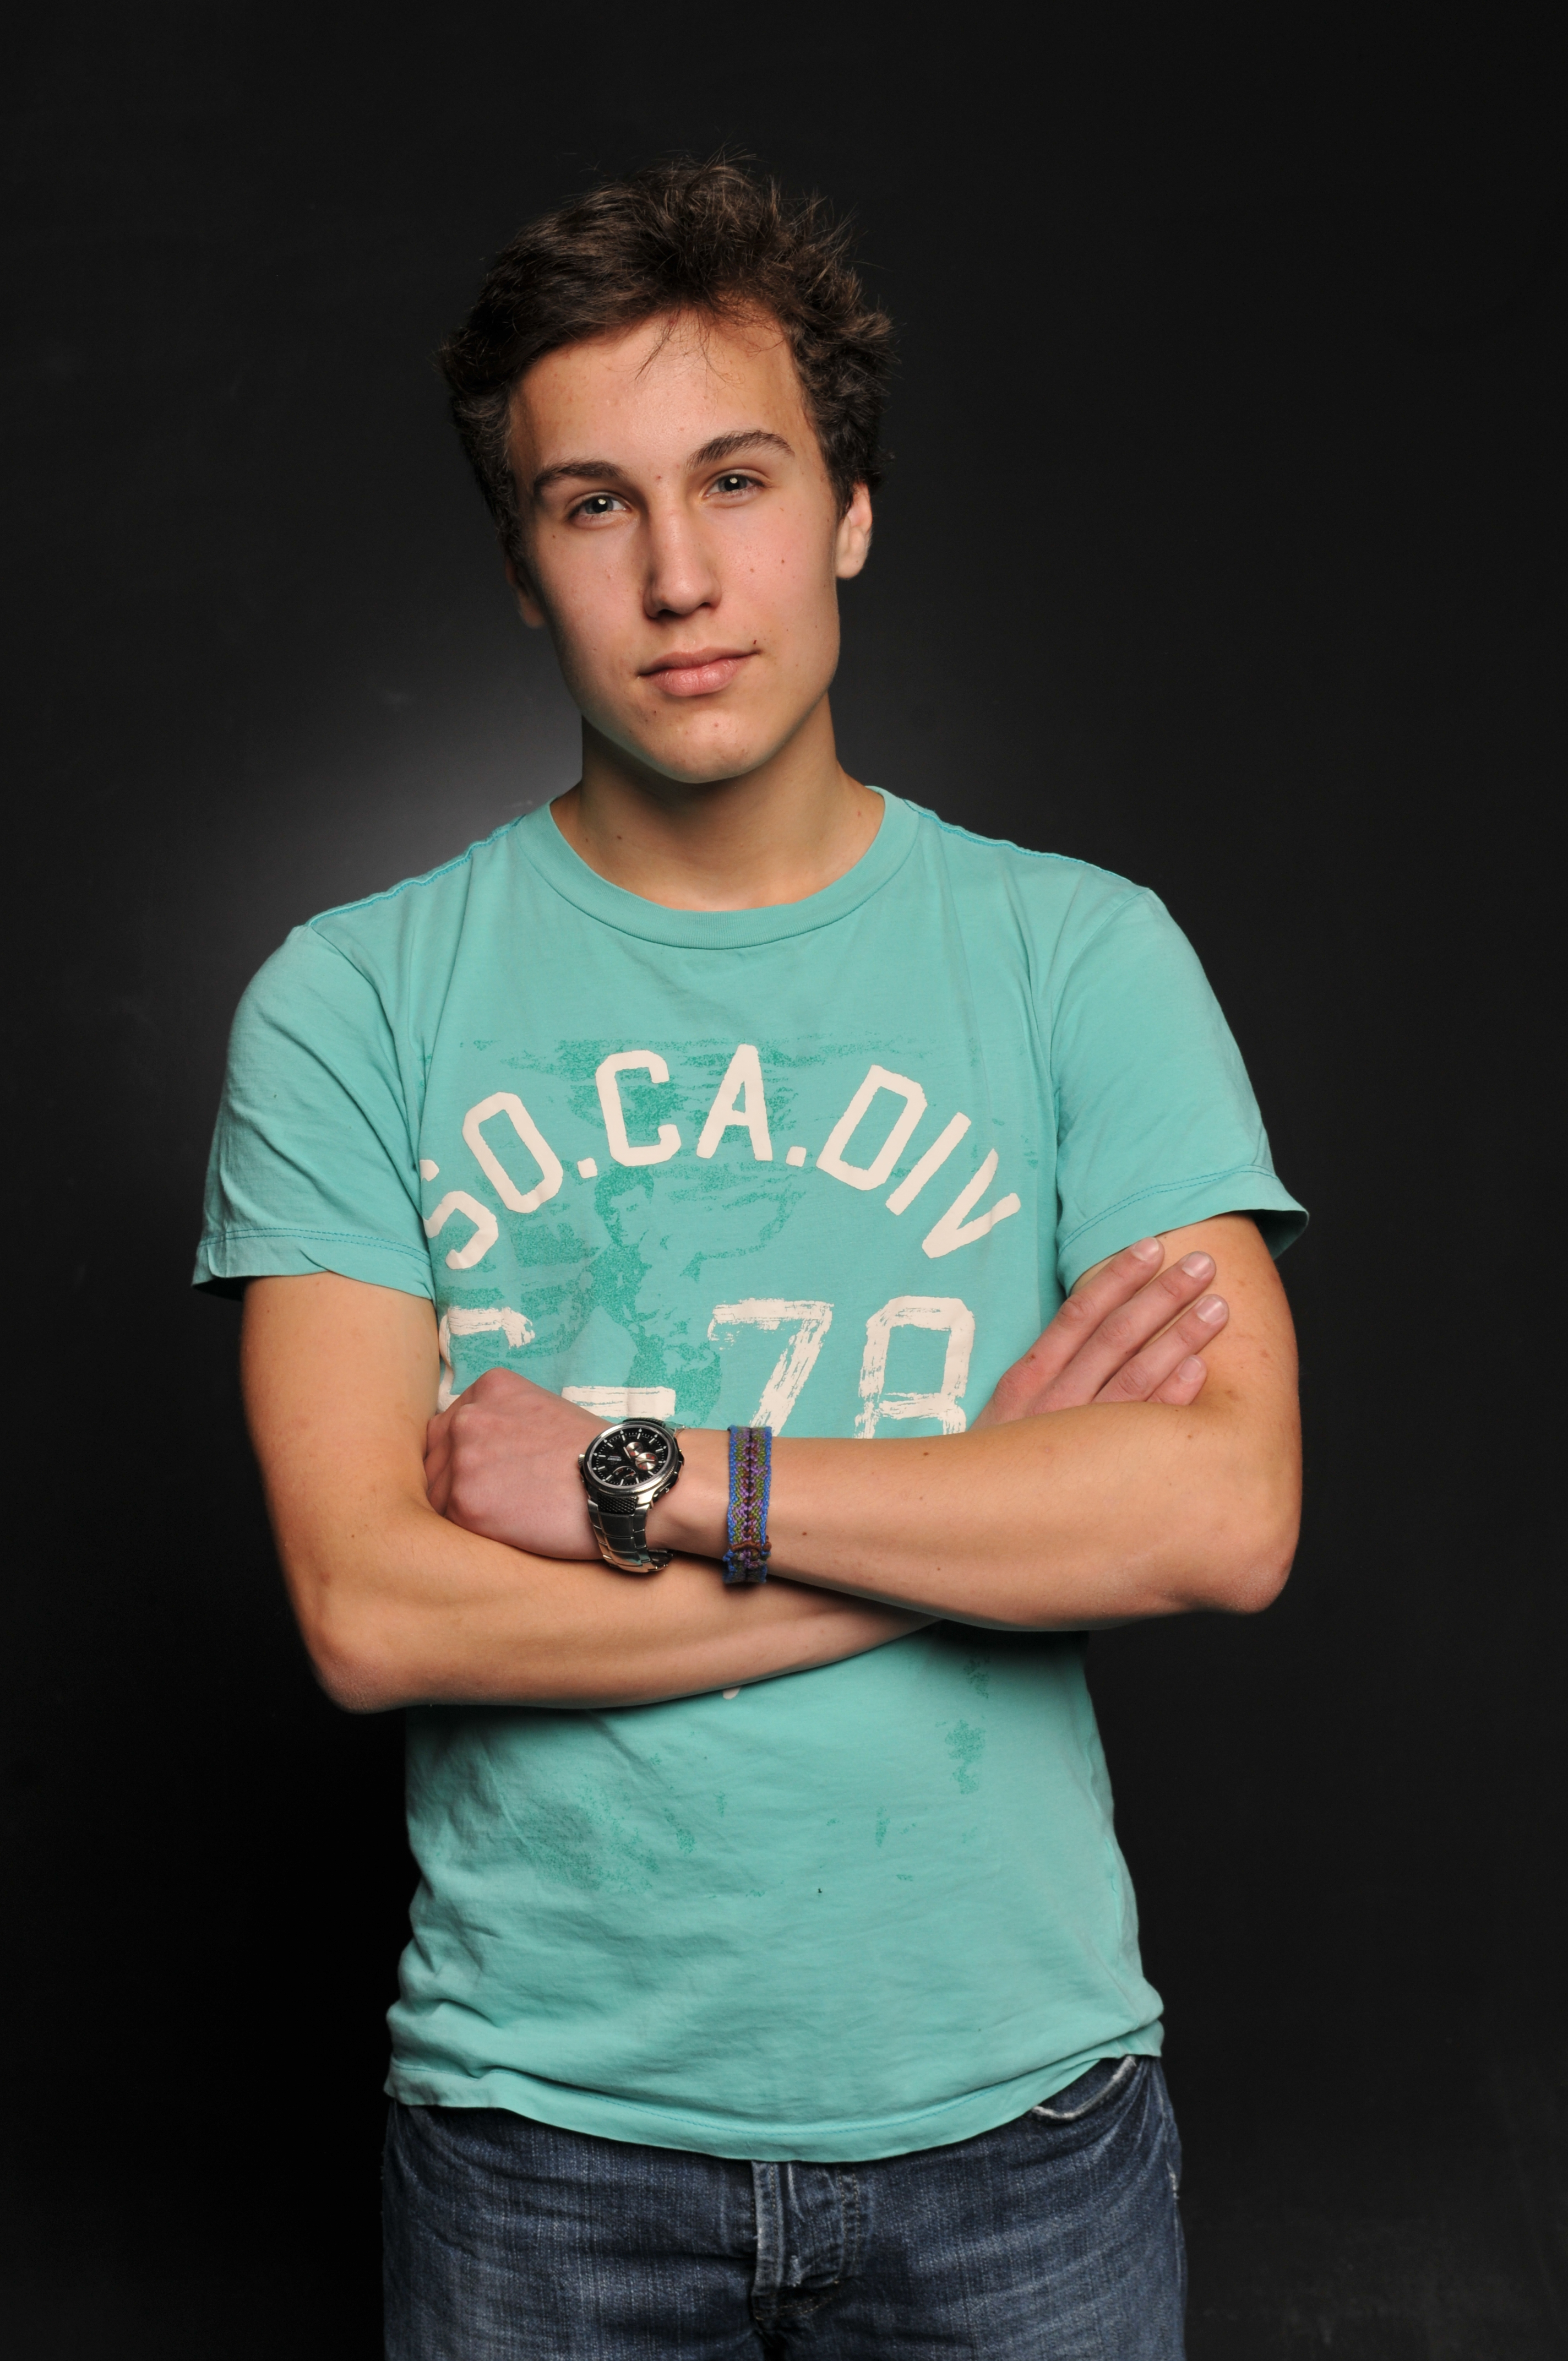
\includegraphics[scale=0.25]{days/29.09.14/images/03}}
          		\caption{Ideas of fixing of moving baskets: 1)Gripper shaped П 2)Gripper with hooks}
				\end{minipage}
			\end{figure}
          
        \end{enumerate}
      \end{enumerate}
    \end{enumerate}
    
	\item Results: 
	\begin{enumerate}
	  \item By the results of discussion were generated ideas that described in sections "Concept of robot", "Strategy" and "Planned steps for creating of robot".      
    \end{enumerate}
    
	\item Tasks for the next cogregations:
	\begin{enumerate}
	  \item Choose the wheels base.
	  
	  \item Choose the optimal sizes of robot.
	  
	  \item Choose the best system of control of balls.
	  
	  \item Choose the most effective way of fixing of moving basket.
	  
    \end{enumerate}
\end{enumerate}
\fillpage


